The main objective of the present Thesis Project is to unravel the role of lncRNAs in two biological scenarios. The first, cell-growth in seven human cell lines (\textbf{Chapter I}: \nameref{sec:ML  model for classification of functional lncRNAs}). The second, after genetically inducing cell-death in \textit{Drosophila} wing imaginal discs (\textbf{Chapter II}: \nameref{sec:results-dme}). Hence, the objectives of this Thesis Project are (see \autoref{fig:thesis-layout} for a general overview of this thesis work):

\begin{enumerate}

\item To harness the richness of ever-growing public available genomic datasets by using nonlinear models, such as tree-based machine learning models, to generate a classifier to unveil functional lncRNAs in the context of cell-growth in human cell lines.

\item To understand the role of lncRNAs during regeneration, using \textit{Drosophila melanogaster} wing imaginal disc as a regeneration-model, to generate a list of lncRNA candidates to perform experimental validations, and unveil their function in the context of regeneration.
  
\end{enumerate}

\begin{figure}[!htb]
  \centering
  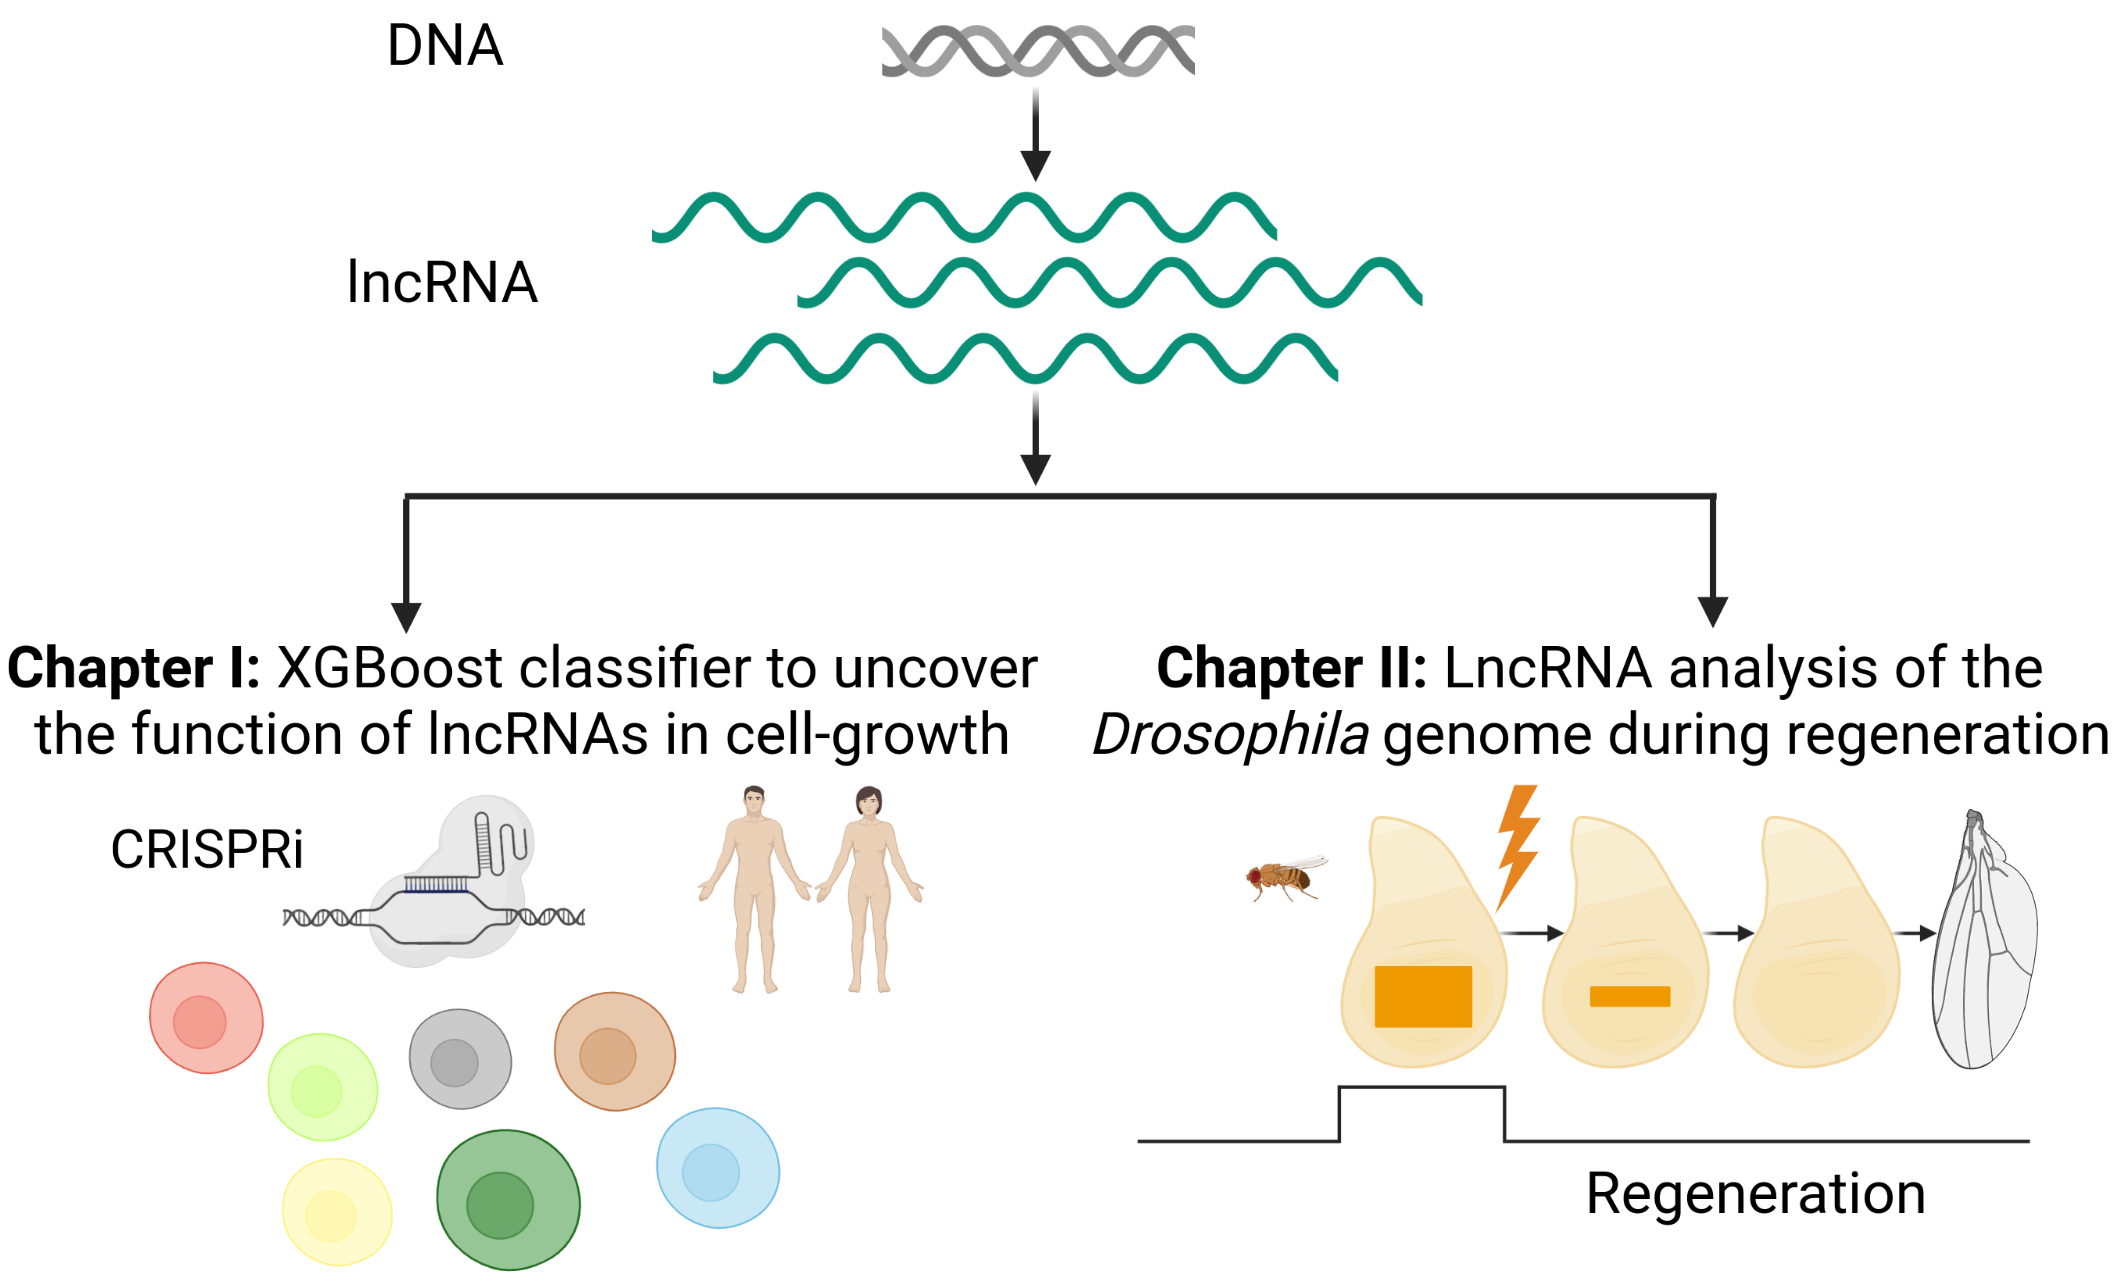
\includegraphics[width=0.85\textwidth]{img/objectives/objectives.png}
  \caption[Thesis outline]{\textbf{Thesis outline}. Graphical abstract of the topics covered in this thesis work.}
  \label{fig:thesis-layout}
\end{figure}

